\section{Introduction}
The blind or visually-impaired persons have the needs to get around just like anyone else, except that they use different methods. In general, they look for “cues” to assess whether a situation may turn nasty. Said Sandy Murillo in her Sandy’s View column [1], a blind person has three common options for mobility:

\begin{enumerate}
  \item A blind cane. It helps the user know when there are tripping hazards such as cracks, poles, etc. The cane is swept from side to side to clear one’s path from obstacles.
  \item A service animal. They received special and extensive training to guide their handlers around obstacles and can also help find things like entrances, escalators, and elevators.
  \item A sighted (or human) guide. A blind person is guided by someone else by holding on to their arm. It is preferred by the blind when in unfamiliar places or if there are large crowds.
\end{enumerate}
However, many blind and visually-impaired find it challenging to acquire the necessary information about their surroundings. For example, a research found that It took significantly longer for them to cross at roundabouts than sighted pedestrians [2]. It’s because they rely on their hearing to determine whether gaps in traffic are crossable.
\newline\newline
Even in a safe environment, say indoor, it could still be challenging for them to describe the surroundings and navigate around.
\newline\newline
To solve these problems, we introduce \textit{IntelliCane}. It’s intelligent in a way that it provides more “cues” to help the user get around. It’s just like being in a self-driving vehicle, you don’t need to worry too much about what’s around you, because sensors did that for you.
\newline\newline
\textit{IntelliCane} uses ultrasonic sensors to help them avoid obstacles on the ground, and a micro camera to recognize and describe surrounding objects. Users can hear the information, including warnings.

\begin{figure}
  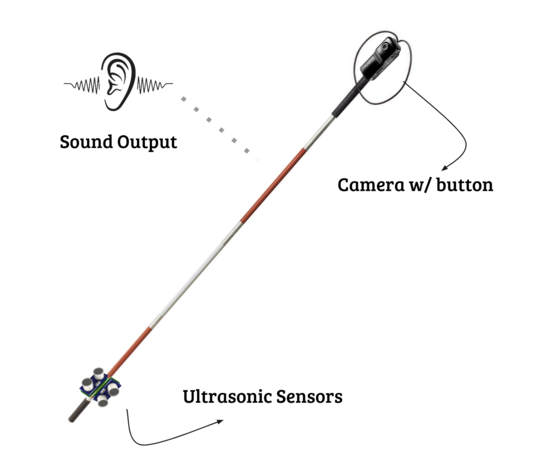
\includegraphics{cane}
  \caption{\textit{IntelliCane} Prototype}
\end{figure}

\section{Related Work}
We researched how the existing work helps to address the problem. As for obstacle detection, smart canes such as the UltraCane or BAT “K” Sonar, use ultrasonic sensors, infrared sensors (e.g., Tom-Pouce), or laser sensors (e.g., LaserCane, Teletac, or Vistac Laser Long Cane) [3]. These sensors increase the detection range and angle. After objects are detected, a smart cane will alert the user of surrounding obstacles. The information is then sent to the user, commonly using a tactile or aural feedback modality. Most of the electronic aids emit vibration alerts rather than audio signals. Some of the smart canes are even more intelligent: they integrate auto-navigation software system like Google Map to help users with visual impairment to navigate through [4].


\section{System Design and Implementation}
\subsection{Components}

\begin{enumerate}
  \item Arduino Uno x 2
  \item Ultrasonic sensor (HC-SR04) x 2
  \item OV2640 2MP Len Camera x 1
  \item Button x 1
\end{enumerate}

\subsection{Obstacle Detection}
We use two ultrasonic sensors to detect obstacles on the blind’s left and right sides. 
To simplify the workflow for the demo, we choose HC-SR04, which provides 2cm - 400cm non-contact measurement function. 
The ranging accuracy can reach to 3mm [5]. Once the obstacle is detected, the distance and direction information will be transmitted and broadcasted in a speaker. 
Then the visually-impaired users can be aware of the incoming obstacle and its relative direction so that he can be prepared and decide where to move in advance.
\newline
However, there might be some problems for such kind of obstacle detection:
\begin{enumerate}
\item The way visual-impaired person uses the cane is normally much more cmplicated than how we test it in the demo.
For instance, they might move the cane super fast to test whether there are anything like obstacles in all directions.
This would make the cane warn all the time because there are always something regarded as obstacles.
\newline
To solve this problem, we might need to improve our warning rules so that such fast movements could be ignored or warnings of a continue movements should be given only once.
\item Are 2 ultrasonic sensors enough for detection of all directions? 
\newline
We doubt it. In the demo, we only used two ultrasonic sensors
to simplify the workflow, but if we are going to build a real product, we will choose to use 2 more sensors for obstacle detection.
\end{enumerate}

\subsection{Surrounding Objects Recognition}
The main goal for surrounding object recognition feature is to enable visual-impaired people who use this smart cane to know the basic information about their environment.
It is not hard to imagine that when entering a new environment, people who cannot see might feel unknown and do need someone else's help to get around.
Therefore, if we can simplify this process by just providing a button to be pressed, visual-impaired people might feel better in an unknown environment.
\newline \newline
In order to recognize objects around the blind, we use an OV2640 2MP Len Camera Shield for Arduino [6] to take pictures and utilize Deep Learning for Computer Vision to detect objects in pictures. After the detection, the voice alert system will notify the blind with possible objects’ names. We also added a button for the blind to control the camera to take pictures so that the recognition mechanism can be more flexible and won’t be annoying. (e.g. blind tends to be walking slowly, in such case, the surrounding environment won’t be changing frequently, which means most of the detected objects will be detected again after a short period time, which makes the system repeats the similar computation and yet outputs the same voice alert.)  
\newline \newline
Considering the computational power of Arduino and the time cost to take pictures using OV2640, we decided that the resolution of the pictures taken is 320*240 in BMP format. As experimented, such resolution is enough for Deep Learning model to detect objects. 
\newline \newline
For the part of object recognition, we tried both online and offline approaches. Google’s online Vision API is powerful and gives many details about detected objects in pictures. However, since our project is for blind and the hardware could be moving around, the network may not be stable and there is also a risk that the online API couldn’t respond timely, we need to make sure no external condition will be intervening the object recognition process. The offline approach is a better way to support the recognition. ImageAI [7] provides out-of-box deep learning model for computer vision. It can be easily integrated into our project and it is also reliable while having a high recognition rate. The model will output detected objects’ names and their possibilities. Currently, our system will alert the blind with all detected objects.

\subsection{System Design}
Considering the limited computational power of Arduino, we decided to separate ultrasonic sensors from the camera. 
One Arduino Uno for ultrasonic sensors, one for the camera. A button is used to control the camera manually. 
The circuit is as the Figure 2 shows. Currently, we connect these two Arduino directly to a laptop using USB and interact with them using Python. 
\newline \newline
Ultrasonic sensors will continuously stream distance measurements for objects to the blind’s left and right to the PC. 
Pictures taken by the camera will be stored as BMP format in PC’s storage and then those pictures will be supplied to ImageAI’s model for object recognition. 

\begin{figure}
  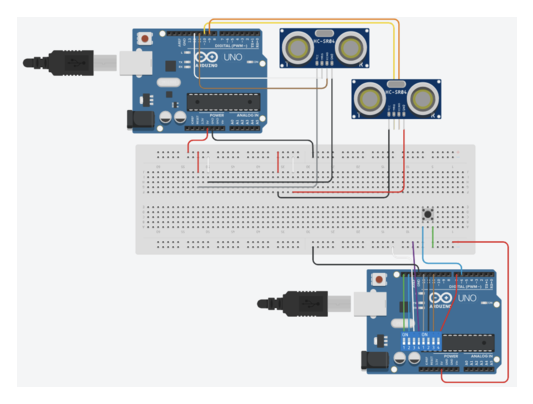
\includegraphics{circuit}
  \caption{Circuit Design}
\end{figure}


\section{Evaluation}
To better analyze the effectiveness and accuracy of our system, we did the following tests.

\subsection{Obstacle Detection Evaluation}
Currently, we are using 2 ultrasonic sensors to detect obstacles from the left side and the right side, so there might be the following situations:

\begin{enumerate}
  \item No obstacles on either side
  \item Obstacles only on the left
  \item Obstacles only on the right
  \item Obstacles on both sides
\end{enumerate}

We tested the obstacle detection system by recording how fast and how accurate the system could provide a result after we put some obstacles around the sensors from different distances, the result of which is shown in Table 1.

\begin{enumerate}
  \item $\pi$ is the parameter we set as the warning distance from the sensor.
  \item Sl is the parameter of how far the obstacles are from the left ultrasonic sensor.
  \item Sr is the parameter of how far the obstacles are from the right ultrasonic sensor.
  \item Al is the result of the left sensor. Al = y means the left sensor warned. Al = n means the left sensor didn’t give any warnings.
  \item Ar is the result of the right sensor. Ar = y means the right sensor warned. Ar = n means the right sensor didn’t give any warnings.
  \item Al is the result of the left sensor. Al = y means the left sensor warned. Al = n means the left sensor didn’t give any warnings.
\end{enumerate}

All units for Pi, Sl, and Sr are cm. $\infty$ means there are no obstacles within the given warning distance Pi.

\begin{table}
  \caption{Obstacle detection evaluation results}
  \label{tab:freq}
  \begin{tabular}{ccccc}
    \toprule
    $\pi$ & Sl & Sr & Al & Ar \\
    \midrule
    10 & $\infty$ & $\infty$ & n & y  \\
    10 & 5 & $\infty$ & y & n  \\
    10 & $\infty$ & 5 & n & y  \\
    10 & 5 & 5 & y & y  \\
    100 & $\infty$ & $\infty$ & n & n  \\
    100 & 50 & $\infty$ & y & n  \\
    100 & $\infty$ & 50 & n & y  \\
    100 & 50 & 50 & y & y  \\
  \bottomrule
\end{tabular}
\end{table}

As the results suggest, the sensor is relatively accurate in terms of distance detection. Also, in the experiments, we found that the sensor was occasionally unresponsive to obstacles that were very close (< 4 cm).

\subsection{Obstacle Recognition Evaluation} 
As ImageAI, which we use as the object recognition framework, provides 3 different well-trained models, we test our image recognition system by changing the distance between objects and the camera using the 3 provided models, the result of which is shown in Table 2.
\begin{enumerate}
  \item M is the parameter of the well-trained models.
  \item O is how many obvious objects are in front of the camera.
  \item D is many obvious objects are recognized by the system including both correctly and wrongly detected objects.
  \item T is the parameter telling how long the recognition process took (unit: seconds).
  \item A is the accuracy of detected objects, which is correctly detected objects / D.
  \item F is the figure showing the test results.
\end{enumerate}

% You can access the test results from this repo:
% https://github.com/geeeeeeeeek/smart-cane/tree/master/arduino/extras/testResult 



\begin{table}
  \caption{Obstacle recognition evaluation results} 
  \label{tab:freq}
  \begin{tabular}{ccccccc}
    \toprule
    Image & M & O & D & T & A & F \\
    \midrule
    Image 1 & RetinaNet & 7 & 4 & 13.00 & 0.57 & Figure 3 \\
    Image 1 & YOLOv3 & 7 & 6 & 20.75 & 0.86 & Figure 4 \\
    Image 1 & TinyYOLOv3 & 7 & 1 & 14.82 & 0.14 & Figure 5  \\
    Image 2 & RetinaNet & 8 & 5 & 15.37 & 0.63 & Figure 6  \\
    Image 2 & YOLOv3 & 8 & 8 (1 false detection) & 24.08 & 0.88 & Figure 7 \\
    Image 2 & TinyYOLOv3 & 8 & 2 & 16.09 & 0.25 & Figure 8 \\
  \bottomrule
\end{tabular}
\end{table}

\section{Conclusion}
The goal of IntelliCane is to help the blind and visually-impaired get around more efficiently and more confidently. To achieve the goal, IntelliCane uses ultrasonic sensors to help avoid obstacles on the ground, and a micro camera to recognize and describe surrounding objects. The design is done and a prototype has been produced. The evaluation shows that both the sensors and the algorithm work as expected.


\begin{figure}
  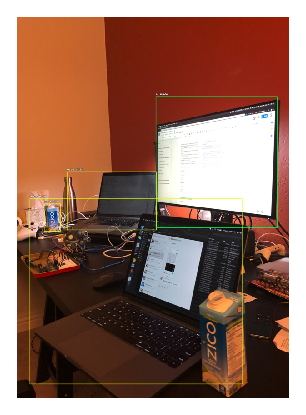
\includegraphics{figure3}
  \caption{Detected Image1 Using RetinaNet}
\end{figure}

\begin{figure}
  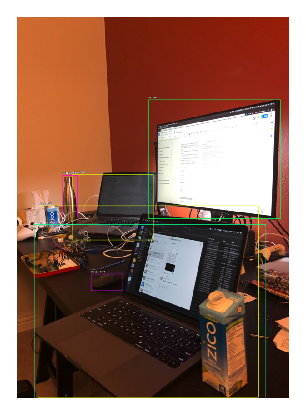
\includegraphics{figure4}
  \caption{Detected Image1 Using YOLOv3}
\end{figure}

\begin{figure}
  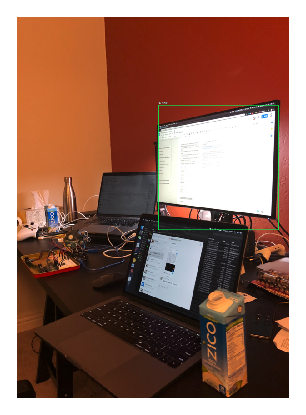
\includegraphics{figure5}
  \caption{Detected Image1 Using TinyYOLOv3}
\end{figure}

\begin{figure}
  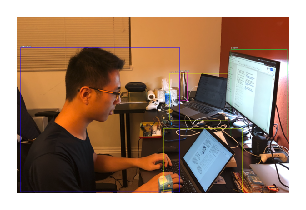
\includegraphics{figure6} 
  \caption{Detected Image2 Using RetinaNet}
\end{figure}

\begin{figure}
  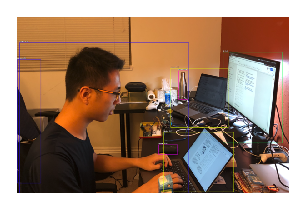
\includegraphics{figure8} 
  \caption{Detected Image2 Using YOLOv3}
\end{figure}

\begin{figure}
  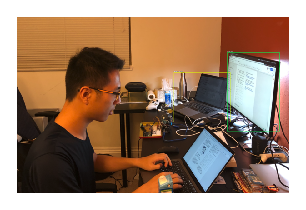
\includegraphics{figure7}
  \caption{Detected Image2 Using TinyYOLOv3}
\end{figure}

\section{References}
[1] “How Do Blind and Visually Impaired People Get Around?”, Sandy Murillo, Sandy’s View, https://chicagolighthouse.org/sandys-view/getting-around/ 
\newline
[2] Geruschat, Duane R., and Shirin E. Hassan. "Driver Behavior in Yielding to Sighted and Blind Pedestrians at Roundabouts." Journal of Visual Impairment and Blindness 99.5 (2005): 286-302.
\newline
[3] “Usability and Design Guidelines of Smart Canes for Users with Visual Impairments”, Sung Yeon Kim and Kwangsu Cho, 
\newline
http://www.ijdesign.org/index.php/IJDesign/article/view/1209/559 
\newline
[4] “Introducing the Revolutionary Smart Cane WeWALK”, WeWalk, https://www.applevis.com/forum/hardware-accessories/introducing-revolutionary-smart-cane-wewalk
\newline
[5] “Ultrasonic Ranging Module HC - SR04”, 
\newline
https://www.mouser.com/ds/2/813/HCSR04-1022824.pdf
\newline
[6] ArduCam, http://www.arducam.com/camera-modules/2mp-ov2640/
\newline
[7] ImageAI, https://github.com/OlafenwaMoses/ImageAI

% Some examples.  A paginated journal article \cite{Abril07}, an enumerated

% \section{References}
% \section{Introduction}


\subsection{Citations}
% Citations to articles~\cite{bowman:reasoning,
% clark:pct, braams:babel, herlihy:methodology},

hhhhh \cite{hardware:hw1:ref1}
\newline

conference proceedings~\cite{clark:pct} or maybe
books \cite{Lamport:LaTeX, salas:calculus} listed
in the Bibliography section of your
article will occur throughout the text of your article.
You should use BibTeX to automatically produce this bibliography;
you simply need to insert one of several citation commands with
a key of the item cited in the proper location in
the \texttt{.tex} file~\cite{Lamport:LaTeX}.
The key is a short reference you invent to uniquely
identify each work; in this sample document, the key is
the first author's surname and a
word from the title.  This identifying key is included
with each item in the \texttt{.bib} file for your article.





